\documentclass[12pt, a4paper]{article}

% ── Packages ──────────────────────────────────────────────────────────────────
\usepackage[margin=2.5cm, top=3cm, bottom=3cm]{geometry}
\usepackage[table]{xcolor}
\usepackage{amsmath}
\usepackage{booktabs}
\usepackage{array}
\usepackage{tabularx}
\usepackage{graphicx}
\usepackage{hyperref}
\usepackage{fancyhdr}
\usepackage{titlesec}
\usepackage{parskip}
\usepackage{enumitem}
\usepackage[letterspace=150]{microtype}
\usepackage{mdframed}
\usepackage{lmodern}
\usepackage{fontenc}
\usepackage{inputenc}
\usepackage{caption}
\usepackage{subcaption}
\usepackage{float}
\usepackage{multirow}
\usepackage{longtable}
\usepackage{tcolorbox}
\tcbuselibrary{skins, breakable}

% ── Colours ───────────────────────────────────────────────────────────────────
\definecolor{ehaBlue}{RGB}{0, 84, 142}
\definecolor{ehaLightBlue}{RGB}{224, 237, 248}
\definecolor{ehaGrey}{RGB}{245, 245, 245}
\definecolor{ehaAccent}{RGB}{0, 153, 118}
\definecolor{ehaRed}{RGB}{192, 57, 43}
\definecolor{ehaAmber}{RGB}{230, 126, 34}
\definecolor{tableHead}{RGB}{0, 84, 142}
\definecolor{tableAlt}{RGB}{240, 248, 255}
\definecolor{mapeGreen}{RGB}{212, 237, 218}
\definecolor{mapeAmber}{RGB}{255, 243, 205}
\definecolor{mapeRed}{RGB}{248, 215, 218}

% ── Hyperlinks ────────────────────────────────────────────────────────────────
\hypersetup{
  colorlinks=true, linkcolor=ehaBlue, urlcolor=ehaBlue,
  pdftitle={Tier 3 Prophet Forecasting Report --- EHA Clinics},
  pdfauthor={Supply Chain Analytics},
}

% ── Header / Footer ───────────────────────────────────────────────────────────
\pagestyle{fancy}
\fancyhf{}
\fancyhead[L]{\small\textcolor{ehaBlue}{\textbf{EHA Clinics} $\mid$ Tier 3 Demand Forecasting Report --- Prophet}}
\fancyhead[R]{\small\textcolor{gray}{May 2026}}
\fancyfoot[C]{\small\textcolor{gray}{\thepage}}
\renewcommand{\headrulewidth}{0.4pt}
\renewcommand{\headrule}{\hbox to\headwidth{\color{ehaBlue}\leaders\hrule height\headrulewidth\hfill}}
\setlength{\headheight}{25.4pt}

% ── Section styling ───────────────────────────────────────────────────────────
\titleformat{\section}{\large\bfseries\color{ehaBlue}}{\thesection.}{0.6em}{}[\titlerule]
\titleformat{\subsection}{\normalsize\bfseries\color{ehaBlue!80!black}}{\thesubsection}{0.6em}{}
\titleformat{\subsubsection}{\small\bfseries\color{ehaBlue!60!black}}{\thesubsubsection}{0.6em}{}
\titlespacing*{\section}{0pt}{1.6em}{0.7em}
\titlespacing*{\subsection}{0pt}{1.1em}{0.4em}
\titlespacing*{\subsubsection}{0pt}{0.9em}{0.3em}

% ── Callout boxes ─────────────────────────────────────────────────────────────
\mdfdefinestyle{keybox}{
  backgroundcolor=ehaLightBlue, linecolor=ehaBlue, linewidth=1pt,
  innerleftmargin=12pt, innerrightmargin=12pt,
  innertopmargin=10pt, innerbottommargin=10pt, roundcorner=4pt,
}
\mdfdefinestyle{warnbox}{
  backgroundcolor=ehaAmber!12, linecolor=ehaAmber, linewidth=1.5pt,
  topline=false, rightline=false, bottomline=false,
  innerleftmargin=12pt, innerrightmargin=12pt,
  innertopmargin=8pt, innerbottommargin=8pt,
}
\mdfdefinestyle{alertbox}{
  backgroundcolor=ehaRed!8, linecolor=ehaRed, linewidth=1.5pt,
  topline=false, rightline=false, bottomline=false,
  innerleftmargin=12pt, innerrightmargin=12pt,
  innertopmargin=8pt, innerbottommargin=8pt,
}
\mdfdefinestyle{greenbox}{
  backgroundcolor=ehaAccent!10, linecolor=ehaAccent, linewidth=1.5pt,
  topline=false, rightline=false, bottomline=false,
  innerleftmargin=12pt, innerrightmargin=12pt,
  innertopmargin=8pt, innerbottommargin=8pt,
}

% ── Table helpers ─────────────────────────────────────────────────────────────
\newcolumntype{L}[1]{>{\raggedright\arraybackslash}p{#1}}
\newcolumntype{C}[1]{>{\centering\arraybackslash}p{#1}}
\newcolumntype{R}[1]{>{\raggedleft\arraybackslash}p{#1}}

% ── Figure caption style ──────────────────────────────────────────────────────
\captionsetup{font=small, labelfont={bf,color=ehaBlue}, labelsep=period,
              skip=6pt, width=0.95\textwidth}

% ── Finding counter ───────────────────────────────────────────────────────────
\newcounter{finding}
\newcommand{\finding}[1]{%
  \stepcounter{finding}%
  \begin{mdframed}[style=greenbox]
  \textbf{Finding \thefinding:} #1
  \end{mdframed}%
}

\begin{document}

% ════════════════════════════════════════════════════════════════════════════════
%  TITLE PAGE
% ════════════════════════════════════════════════════════════════════════════════
\begin{titlepage}
  \pagecolor{ehaBlue}\color{white}
  \vspace*{1.8cm}

  {\fontsize{10}{12}\selectfont\MakeUppercase{\textls[100]{Analytical Report}}}\\[0.5em]
  {\fontsize{26}{32}\selectfont\bfseries Tier 3 Demand Forecasting:\\[0.3em]
   Facebook Prophet with Nigerian\\[0.3em]
   Holiday Regressors}\\[1.2em]
  \textcolor{ehaAccent}{\rule{6cm}{2pt}}\\[1.2em]

  {\large Procurement Demand Forecasting Initiative}\\[0.4em]
  {\normalsize EHA Clinics $\cdot$ Supply Chain Analytics}\\[2.5cm]

  \begin{tabular}{@{}ll}
    \textbf{Document Version}  & 1.0 \\[0.4em]
    \textbf{Date}              & May 2, 2026 \\[0.4em]
    \textbf{Data source}       & Odoo ERP (exported CSV) \\[0.4em]
    \textbf{Training window}   & January 2021 -- December 2023 \\[0.4em]
    \textbf{Validation window} & January 2024 -- June 2024 \\[0.4em]
    \textbf{Status}            & Final --- Q3 Evaluation \\
  \end{tabular}

  \vfill
  {\small\textcolor{white!70!ehaBlue}
    {This report documents the implementation and evaluation of Tier 3
     (Facebook Prophet) forecasting models with Nigerian holiday and
     procurement-cycle regressors across all 15 eligible
     category-facility pairs. It presents the Q3 MAPE assessment,
     the improvement achieved over the Tier 1 \& 2 baseline, and
     identifies which pairs have met the KPI target of MAPE
     $\leq 20\%$, along with those requiring escalation to Tier 4
     (machine learning methods).}}
\end{titlepage}
\pagecolor{white}\color{black}

% ════════════════════════════════════════════════════════════════════════════════
%  EXECUTIVE SUMMARY
% ════════════════════════════════════════════════════════════════════════════════
\newpage

\begin{mdframed}[style=keybox]
\textbf{\large Executive Summary}\\[0.6em]
This report presents the results of the Tier 3 forecasting phase of the
EHA Clinics Procurement Demand Forecasting Initiative. Facebook Prophet
--- a decomposable Bayesian time-series model --- was applied to all
\textbf{15 eligible category-facility pairs} with a purpose-built Nigerian
holiday and procurement-cycle regressor calendar. Models were trained on
the January 2021--December 2023 window, hyperparameters were optimised via
a 9-combination walk-forward cross-validation grid, and final performance
was evaluated against January--June 2024 actuals.\\[0.5em]

Seven key conclusions emerge from this evaluation:

\begin{enumerate}[leftmargin=1.5em, itemsep=3pt]
  \item \textbf{Prophet materially outperforms Tier 1 and Tier 2 models
        on the majority of pairs.} Its explicit Fourier-series seasonality
        decomposition and holiday-effect regression address the primary
        structural weaknesses identified in classical models (SARIMA
        instability, ETS rigidity on multiplicative seasonal patterns).

  \item \textbf{The Harmattan season regressor (Nov--Feb) is the single
        most impactful domain-specific feature.} OTC Drugs and Prescription
        Medications at anchor facilities show a clear demand elevation
        during the Harmattan dry season that Tier 2 models partially captured
        but Prophet explicitly encodes.

  \item \textbf{Nigerian Islamic holiday regressors (Eid al-Fitr, Eid
        al-Adha) capture procurement pause-and-restock patterns.}
        These two events create operational disruptions --- reduced
        ordering in the preceding weeks and elevated restocking in the
        following month --- that Prophet's holiday window mechanism
        can account for.

  \item \textbf{Year-end budget-flush regressors (Nov--Dec) improve
        accuracy on categories with programme or budget-driven procurement
        spikes.} Laboratory Consumables and Medical Consumables at anchor
        facilities both show December procurement elevation consistent with
        fiscal year-end spending.

  \item \textbf{Hyperparameter tuning reveals that sparse, intermittent
        series benefit from low changepoint flexibility} (changepoint prior
        scale $\leq 0.05$), while categories with clear trend evolution
        (Rx Medications at Asba) benefit from higher flexibility
        (scale $\geq 0.1$).

  \item \textbf{Laboratory Consumables remains a special case.}
        The all-zero validation window at Asba is a known data gap that
        prevents MAPE evaluation. Kano Lamido's extreme bulk-event
        pattern yields high error regardless of model, pending
        supply-chain-level root cause resolution.

  \item \textbf{Pairs that still do not meet the $\leq 20\%$ MAPE target
        after Tier 3 are escalated to Tier 4 (XGBoost / Random Forest)}
        with a recommendation to incorporate consultation-volume and
        external demand-driver features before model fitting.
\end{enumerate}
\end{mdframed}

\newpage
\tableofcontents
\newpage

% ════════════════════════════════════════════════════════════════════════════════
%  1. INTRODUCTION
% ════════════════════════════════════════════════════════════════════════════════
\section{Introduction}

\subsection{Purpose and Context}

This report is the third in a series documenting the EHA Clinics
Procurement Demand Forecasting Initiative. It follows:

\begin{itemize}[leftmargin=1.5em, itemsep=3pt]
  \item \textbf{Forecasting Scope and Modelling Approach} (Concept Note,
        April 2026) --- which defined the tiered modelling strategy,
        six pilot facilities, nine commodity categories, and the
        KPI target of MAPE $\leq 20\%$.

  \item \textbf{Exploratory Data Analysis Report} (April 2026) ---
        which characterised demand patterns, identified the Kano
        Independence Road bulk stock-load anomaly (September 2021),
        and classified pairs by data readiness (Tier A/B/C).

  \item \textbf{Tier 1 \& 2 Demand Forecasting Report} (May 2026) ---
        which established the Q2 MAPE baseline across five classical
        models, found that no pair met the $\leq 20\%$ target, and
        escalated all 15 eligible pairs to Tier 3 (Prophet).
\end{itemize}

The present document reports the \textbf{Tier 3 evaluation}: Facebook
Prophet with a domain-specific Nigerian holiday and procurement-cycle
regressor calendar, systematic hyperparameter tuning via walk-forward
cross-validation, and final hold-out validation against the
January--June 2024 window.

\subsection{Why Prophet at Tier 3}

The Tier 1 and Tier 2 evaluation identified four structural failure
modes in classical models that Prophet is specifically designed to
address:

\vspace{0.5em}
\noindent
\begin{tabularx}{\textwidth}{@{} L{4.2cm} X @{}}
  \toprule
  \rowcolor{tableHead}
  \textcolor{white}{\textbf{Failure mode (Tier 1/2)}} &
  \textcolor{white}{\textbf{Prophet's response}} \\
  \midrule
  SARIMA instability on sparse series
  (MAPEs $>$1,000\% on 4 pairs) &
    Piecewise linear trend with automatic changepoint detection requires
    no differencing; never produces explosive forecasts on series
    with zero-valued gaps. \\
  \rowcolor{tableAlt}
  ETS / Theta miss Q4 Harmattan OTC peak &
    Yearly Fourier seasonality captures amplitude and phase; a binary
    Harmattan regressor (Nov--Feb) adds an explicit demand-elevation
    term that ETS's additive seasonal component underestimates. \\
  Vaccines miss immunisation programme
  procurement cycle timing &
    Nigerian public holidays and programme event dates are passed as
    Prophet holiday regressors, allowing the model to attribute
    procurement spikes to their causal event rather than treating
    them as unexplained noise. \\
  \rowcolor{tableAlt}
  100\% MAPE floor on intermittent series
  (model predicts non-zero, actual is zero) &
    Prophet's additive regression framework with zero-clipping of
    forecasts handles sparsity more gracefully than ARMA-family models;
    the holiday window mechanism can suppress forecast elevations in
    months where low procurement is systematically expected. \\
  \bottomrule
\end{tabularx}

\subsection{KPI and Evaluation Protocol}

The KPI from management remains unchanged:

\begin{mdframed}[style=keybox]
\textit{``Achieve MAPE $\leq 20\%$ for critical health commodities across
pilot facilities by Q3 2026.''}
\end{mdframed}

\vspace{0.5em}

MAPE is computed only over months with non-zero actual procurement
(to avoid division by zero on sparse series):

\[
  \text{MAPE} = \frac{1}{n_{\text{nz}}} \sum_{t\,:\,A_t>0}
  \left| \frac{A_t - F_t}{A_t} \right| \times 100
\]

where $n_{\text{nz}}$ is the count of non-zero validation months.
All forecasts are clipped to zero before MAPE computation to prevent
negative forecasts from inflating error.

The evaluation protocol is identical to Tier 2:
\begin{itemize}[leftmargin=1.5em, itemsep=3pt]
  \item \textbf{Walk-forward CV} (Fold 1: Jan~2021--Dec~2022 train /
        Jan--Jun~2023 validate; Fold 2: Jan~2021--Jun~2023 train /
        Jul--Dec~2023 validate) --- used for hyperparameter selection.
  \item \textbf{Final hold-out} --- full training window (Jan~2021--Dec~2023)
        fitted with best hyperparameters per pair; validated against
        Jan--Jun 2024 actuals.
\end{itemize}

% ════════════════════════════════════════════════════════════════════════════════
%  2. DATA PREPARATION
% ════════════════════════════════════════════════════════════════════════════════
\section{Data Preparation}

\subsection{Filtering Pipeline}

The Tier 3 analysis applies the identical filtering pipeline as Tier 2,
ensuring full comparability of MAPE results:

\begin{enumerate}[leftmargin=1.5em, itemsep=3pt]
  \item Retain only \texttt{state = done} records.
  \item Require \texttt{product\_qty > 0} and \texttt{price\_subtotal} $\geq$ 0.
  \item Restrict to nine in-scope commodity categories and six pilot
        facilities.
  \item Exclude Kano Independence Road 2021 bulk event (365 records,
        Sep~2021 stock-load exercise: 258,470 units).
  \item Aggregate to monthly totals per category-facility pair and
        zero-fill all months within Jan~2021--Jun~2024, yielding a
        complete 42-month matrix.
\end{enumerate}

Final dataset: \textbf{8,458 records} across \textbf{6 facilities},
\textbf{9 categories}, covering \textbf{45 pairs} $\times$ \textbf{42 months}.

\subsection{Pair Classification}

The Tier A/B/C readiness classification is carried forward from Tier 2:

\vspace{0.5em}
\noindent
\begin{tabularx}{\textwidth}{@{} C{1.6cm} L{3.2cm} R{1.8cm} X @{}}
  \toprule
  \rowcolor{tableHead}
  \textcolor{white}{\textbf{Tier}} &
  \textcolor{white}{\textbf{Criterion}} &
  \textcolor{white}{\textbf{Pairs}} &
  \textcolor{white}{\textbf{Treatment}} \\
  \midrule
  \textbf{A} & $\geq$24 non-zero months & 13 & Full Prophet pipeline \\
  \rowcolor{tableAlt}
  \textbf{B} & 12--23 non-zero months & 2 &
    Full Prophet pipeline (same as Tier A; Prophet handles short series
    robustly due to Bayesian priors) \\
  \textbf{C} & $<$12 non-zero months & 28 &
    Excluded; fixed-interval ordering continues to apply \\
  \bottomrule
\end{tabularx}

\vspace{0.5em}
\textbf{15 pairs} proceed to Tier 3 modelling (13 Tier A + 2 Tier B).

% ════════════════════════════════════════════════════════════════════════════════
%  3. NIGERIAN HOLIDAY & PROCUREMENT CALENDAR
% ════════════════════════════════════════════════════════════════════════════════
\section{Nigerian Holiday \& Procurement Event Calendar}

\subsection{Rationale for Event Regressors}

A fundamental insight from the EDA was that demand at EHA Clinics is
\textbf{event-driven} as much as it is cyclically seasonal. Three
distinct event mechanisms were identified:

\begin{enumerate}[leftmargin=1.5em, itemsep=5pt]
  \item \textbf{Nigerian public holidays} --- most critically, Eid al-Fitr
        and Eid al-Adha, which create 3--5 day operational pauses at
        facilities serving Kano (predominantly Muslim population).
        Procurement orders placed immediately before these holidays spike
        as facilities stock up; order activity drops to near-zero during
        the holiday window itself.

  \item \textbf{The Harmattan dry season} (November through February)
        is Nigeria's arid, dusty, and cold-night season. It systematically
        elevates demand for respiratory medications (salbutamol, antihistamines),
        dermatological products, and OTC analgesics. This is a recurring,
        predictable demand elevation that is \textit{not} captured by
        standard yearly Fourier seasonality, which distributes amplitude
        smoothly across the calendar.

  \item \textbf{Year-end fiscal-cycle procurement} (November--December)
        reflects EHA Clinics' budget calendar. Uncommitted supply-chain
        budget is often consumed in Q4, producing a consistent procurement
        surge in November and December that is unrelated to patient demand
        but is a real and predictable procurement pattern.
\end{enumerate}

\subsection{Holiday Calendar Construction}

Prophet receives holiday event information as a dataframe with columns
\texttt{ds} (date) and \texttt{holiday} (event name). For monthly data,
all holiday dates are \textbf{snapped to the first day of their calendar
month}, matching the time series frequency. This means Prophet attributes
the holiday effect to the procurement month in which the event falls.

\vspace{0.5em}
\noindent
\begin{tabularx}{\textwidth}{@{} L{4.2cm} L{2.2cm} X @{}}
  \toprule
  \rowcolor{tableHead}
  \textcolor{white}{\textbf{Event}} &
  \textcolor{white}{\textbf{Type}} &
  \textcolor{white}{\textbf{Procurement mechanism}} \\
  \midrule
  New Year's Day (Jan 1) & Fixed & Year-start restocking and budget
    release for the new fiscal year \\
  \rowcolor{tableAlt}
  Democracy Day (Jun 12) & Fixed & Minor; small operational disruption at
    government-linked facilities \\
  Independence Day (Oct 1) & Fixed & Q4 budget activation; October marks
    the start of high-spending season \\
  \rowcolor{tableAlt}
  Christmas / Boxing Day (Dec 25--26) & Fixed & Year-end consumption spike;
    elevated OTC demand; final budget spending \\
  Eid al-Fitr & Islamic
    (variable) & Pre-holiday ordering surge followed by multi-day
    operational pause; restocking in the following month. \\
  \rowcolor{tableAlt}
  Eid al-Adha & Islamic
    (variable) & Same mechanism as Eid al-Fitr but with a longer
    sacrifice/slaughter period that extends the demand disruption window \\
  \bottomrule
\end{tabularx}
\vspace{0.3em}
\captionof{table}{Holiday events encoded in the Prophet regressor calendar.
All dates are snapped to month-start before passing to the model.}
\label{tab:holidays}

\subsubsection{Accurate Eid Dates (2021--2024)}

Islamic holidays follow the lunar Hijri calendar and therefore shift
by approximately 11 days earlier each Gregorian year. The dates used
in this analysis are:

\vspace{0.4em}
\noindent
\begin{tabularx}{\textwidth}{@{} C{1.5cm} C{3.5cm} C{3.5cm} @{}}
  \toprule
  \rowcolor{tableHead}
  \textcolor{white}{\textbf{Year}} &
  \textcolor{white}{\textbf{Eid al-Fitr}} &
  \textcolor{white}{\textbf{Eid al-Adha}} \\
  \midrule
  2021 & 13 May 2021 & 20 July 2021 \\
  \rowcolor{tableAlt}
  2022 & 2 May 2022  & 9 July 2022  \\
  2023 & 21 April 2023 & 28 June 2023 \\
  \rowcolor{tableAlt}
  2024 & 10 April 2024 & 16 June 2024 \\
  \bottomrule
\end{tabularx}
\vspace{0.3em}
\captionof{table}{Eid al-Fitr and Eid al-Adha dates used as Prophet holiday
regressors. Dates are snapped to month-start in the model.}

\subsection{Custom Monthly Regressors}

Two additional domain-specific regressors are added directly to the
Prophet model via \texttt{add\_regressor()}, as binary monthly indicators:

\vspace{0.5em}
\noindent
\begin{tabularx}{\textwidth}{@{} L{3.2cm} L{3.0cm} X @{}}
  \toprule
  \rowcolor{tableHead}
  \textcolor{white}{\textbf{Regressor}} &
  \textcolor{white}{\textbf{Active months}} &
  \textcolor{white}{\textbf{Procurement rationale}} \\
  \midrule
  \texttt{harmattan} &
    November, December, January, February &
    Harmattan dry season elevates respiratory, dermatological, and OTC
    analgesic demand. OTC Drugs showed a clear Q4 peak in EDA Figure 7
    (seasonality analysis), consistent with Harmattan onset. \\
  \rowcolor{tableAlt}
  \texttt{budget\_flush} &
    November, December &
    EHA Clinics' fiscal year-end procurement surge as uncommitted supply
    budget is spent. Observed in the EDA as a December elevation across
    multiple categories at both Asba and Kano Lamido. \\
  \bottomrule
\end{tabularx}
\vspace{0.3em}
\captionof{table}{Custom binary monthly regressors added to all Prophet fits.}
\label{tab:regressors}

% ════════════════════════════════════════════════════════════════════════════════
%  4. PROPHET MODEL CONFIGURATION
% ════════════════════════════════════════════════════════════════════════════════
\section{Prophet Model Configuration}

\subsection{Mathematical Formulation}

Facebook Prophet decomposes the demand time series $y(t)$ into four
additive components:

\[
  y(t) = g(t) + s(t) + h(t) + \sum_{j} \beta_j x_j(t) + \varepsilon_t
\]

where:
\begin{itemize}[leftmargin=1.5em, itemsep=4pt]
  \item $g(t)$ is the \textbf{trend component} --- a piecewise linear
        function with automatic changepoint detection. Trend breakpoints
        are drawn from a sparse prior with scale controlled by the
        \texttt{changepoint\_prior\_scale} hyperparameter.

  \item $s(t)$ is the \textbf{seasonality component} --- a Fourier-series
        approximation of the seasonal signal with period $P = 12$ months
        for yearly seasonality. For a series of order $N$ harmonics:
        \[
          s(t) = \sum_{n=1}^{N} \left[
            a_n \cos\!\left(\frac{2\pi n t}{P}\right) +
            b_n \sin\!\left(\frac{2\pi n t}{P}\right)
          \right]
        \]
        The Fourier coefficients $a_n, b_n$ are estimated jointly with
        the trend and holiday parameters. Their scale is controlled by
        \texttt{seasonality\_prior\_scale}.

  \item $h(t)$ is the \textbf{holiday component} --- a set of
        indicator regressors corresponding to the Nigerian holiday
        calendar (Table~\ref{tab:holidays}). Each holiday contributes an
        additive demand shift; the magnitude of these shifts is controlled
        by \texttt{holidays\_prior\_scale}.

  \item $\sum_j \beta_j x_j(t)$ represents \textbf{custom regressors}:
        the \texttt{harmattan} (Nov--Feb) and \texttt{budget\_flush}
        (Nov--Dec) binary indicators. Their coefficients $\beta_j$ are
        estimated as part of the model fit.

  \item $\varepsilon_t \sim \mathcal{N}(0, \sigma^2)$ is the residual
        error term, handled by Prophet's Bayesian MCMC / MAP estimation
        via CmdStan.
\end{itemize}

\subsection{Configuration Choices}

\vspace{0.4em}
\noindent
\begin{tabularx}{\textwidth}{@{} L{4.8cm} L{3cm} X @{}}
  \toprule
  \rowcolor{tableHead}
  \textcolor{white}{\textbf{Parameter}} &
  \textcolor{white}{\textbf{Value}} &
  \textcolor{white}{\textbf{Justification}} \\
  \midrule
  \texttt{yearly\_seasonality} & \texttt{True} &
    Captures Harmattan Q4 peak and annual programme procurement cycles \\
  \rowcolor{tableAlt}
  \texttt{weekly\_seasonality} & \texttt{False} &
    Time series is monthly; no weekly signal is present \\
  \texttt{daily\_seasonality} & \texttt{False} &
    Time series is monthly; no daily signal is present \\
  \rowcolor{tableAlt}
  \texttt{seasonality\_mode} & \texttt{additive} &
    Additive mode is required for series with zero-valued months.
    Multiplicative mode applies a log-transform that breaks on exact
    zeros, which are present in the training data for most pairs. \\
  \texttt{holidays} & NG calendar &
    Nigerian public and Islamic holiday dataframe (Table~\ref{tab:holidays}) \\
  \rowcolor{tableAlt}
  \texttt{holidays\_prior\_scale} & 1.0 (fixed) &
    Default value; not included in grid search to limit search space \\
  \texttt{add\_regressor} & \texttt{harmattan}, \newline \texttt{budget\_flush} &
    Domain-specific binary monthly indicators (Table~\ref{tab:regressors}) \\
  \rowcolor{tableAlt}
  Forecast clipping & $\hat{y}(t) \leftarrow \max(\hat{y}(t), 0)$ &
    Prevents negative procurement forecasts, which are physically
    impossible \\
  \bottomrule
\end{tabularx}
\vspace{0.3em}
\captionof{table}{Prophet model configuration parameters and justifications.}

\subsection{Why Additive Seasonality Mode}

The choice of \texttt{seasonality\_mode='additive'} requires explicit
justification, as multiplicative mode can better represent demand signals
where seasonal swings are proportional to the series level (e.g., a
facility with higher average throughput also sees larger absolute seasonal
peaks).

For this dataset, however, additive mode is the only viable option
because:

\begin{itemize}[leftmargin=1.5em, itemsep=4pt]
  \item \textbf{Training series contain zero-valued months.} Prophet's
        multiplicative mode applies a log-transform to the target variable
        $y(t)$. When $y(t) = 0$, $\log(0) = -\infty$, causing numerical
        failure during Stan model fitting. This is not a corner case ---
        most category-facility pairs have 5--15 zero months in the
        36-month training window.

  \item \textbf{Additive mode is sufficiently expressive for this data.}
        The seasonal amplitudes at EHA Clinics facilities are not strongly
        proportional to baseline levels. The OTC Q4 Harmattan peak, for
        example, produces absolute demand elevations of a roughly constant
        size regardless of the facility's throughput level.

  \item \textbf{The Harmattan and budget\_flush regressors partially
        substitute for multiplicative seasonality.} By explicitly encoding
        the Q4 demand elevation as a binary indicator, the additive model
        achieves the same effective signal amplification without requiring
        multiplicative scaling.
\end{itemize}

% ════════════════════════════════════════════════════════════════════════════════
%  5. HYPERPARAMETER TUNING
% ════════════════════════════════════════════════════════════════════════════════
\section{Hyperparameter Tuning}

\subsection{Tuning Parameters and Grid}

Two Prophet hyperparameters were tuned per category-facility pair:

\vspace{0.5em}
\noindent
\begin{tabularx}{\textwidth}{@{} L{5cm} L{5cm} X @{}}
  \toprule
  \rowcolor{tableHead}
  \textcolor{white}{\textbf{Parameter}} &
  \textcolor{white}{\textbf{Values tested}} &
  \textcolor{white}{\textbf{Effect}} \\
  \midrule
  \texttt{changepoint\_prior\_scale} &
    0.01,\; 0.05,\; 0.1,\; 0.3 &
    Controls how flexible the piecewise linear trend is. Larger values
    allow more trend breakpoints; smaller values produce a smoother,
    less reactive trend. \\
  \rowcolor{tableAlt}
  \texttt{seasonality\_prior\_scale} &
    1.0,\; 5.0,\; 10.0 &
    Controls how closely the Fourier-series seasonality fits seasonal
    patterns in the training data. Larger values allow the seasonality
    to be more complex and tightly fitted. \\
  \bottomrule
\end{tabularx}

\vspace{0.5em}
Full Cartesian product: $4 \times 3 = \mathbf{9}$ combinations per pair.
Across 15 pairs and 2 CV folds: $9 \times 15 \times 2 = \mathbf{270}$
total Prophet model fits during the tuning phase.

\subsection{Tuning Protocol}

\begin{enumerate}[leftmargin=1.5em, itemsep=5pt]
  \item For each category-facility pair $p$ and each parameter
        combination $\theta$, fit Prophet on the fold training data
        and compute the 6-month forecast MAPE on the fold validation data.

  \item Average the MAPE across the two CV folds:
        $\overline{\text{MAPE}}_p(\theta) =
        \tfrac{1}{2}(\text{MAPE}_{p,1}(\theta) + \text{MAPE}_{p,2}(\theta))$

  \item Select $\theta^*_p = \arg\min_\theta \overline{\text{MAPE}}_p(\theta)$
        as the best parameter set for pair $p$.

  \item Fit the final model for pair $p$ using $\theta^*_p$ on the
        complete training window (Jan~2021--Dec~2023).

  \item Evaluate final model performance on the hold-out validation
        window (Jan--Jun~2024).
\end{enumerate}

\begin{mdframed}[style=warnbox]
\textbf{Tuning independence note:} Hyperparameter selection is performed
\textit{per pair}, not globally. This reflects the heterogeneous demand
structures across category-facility combinations: the optimal changepoint
flexibility for Vaccines at Kano Lamido (a smooth, programme-driven series)
is expected to differ materially from that for Injections at Asba (a
volatile, procedure-driven series). A single global hyperparameter set
would systematically underfit one type and overfit the other.
\end{mdframed}

\subsection{Tuning Results}

Figure~\ref{fig:tuning} presents the best cross-validation MAPE per pair
from the hyperparameter grid search, alongside the distribution of selected
\texttt{changepoint\_prior\_scale} values.

\begin{figure}[H]
  \centering
  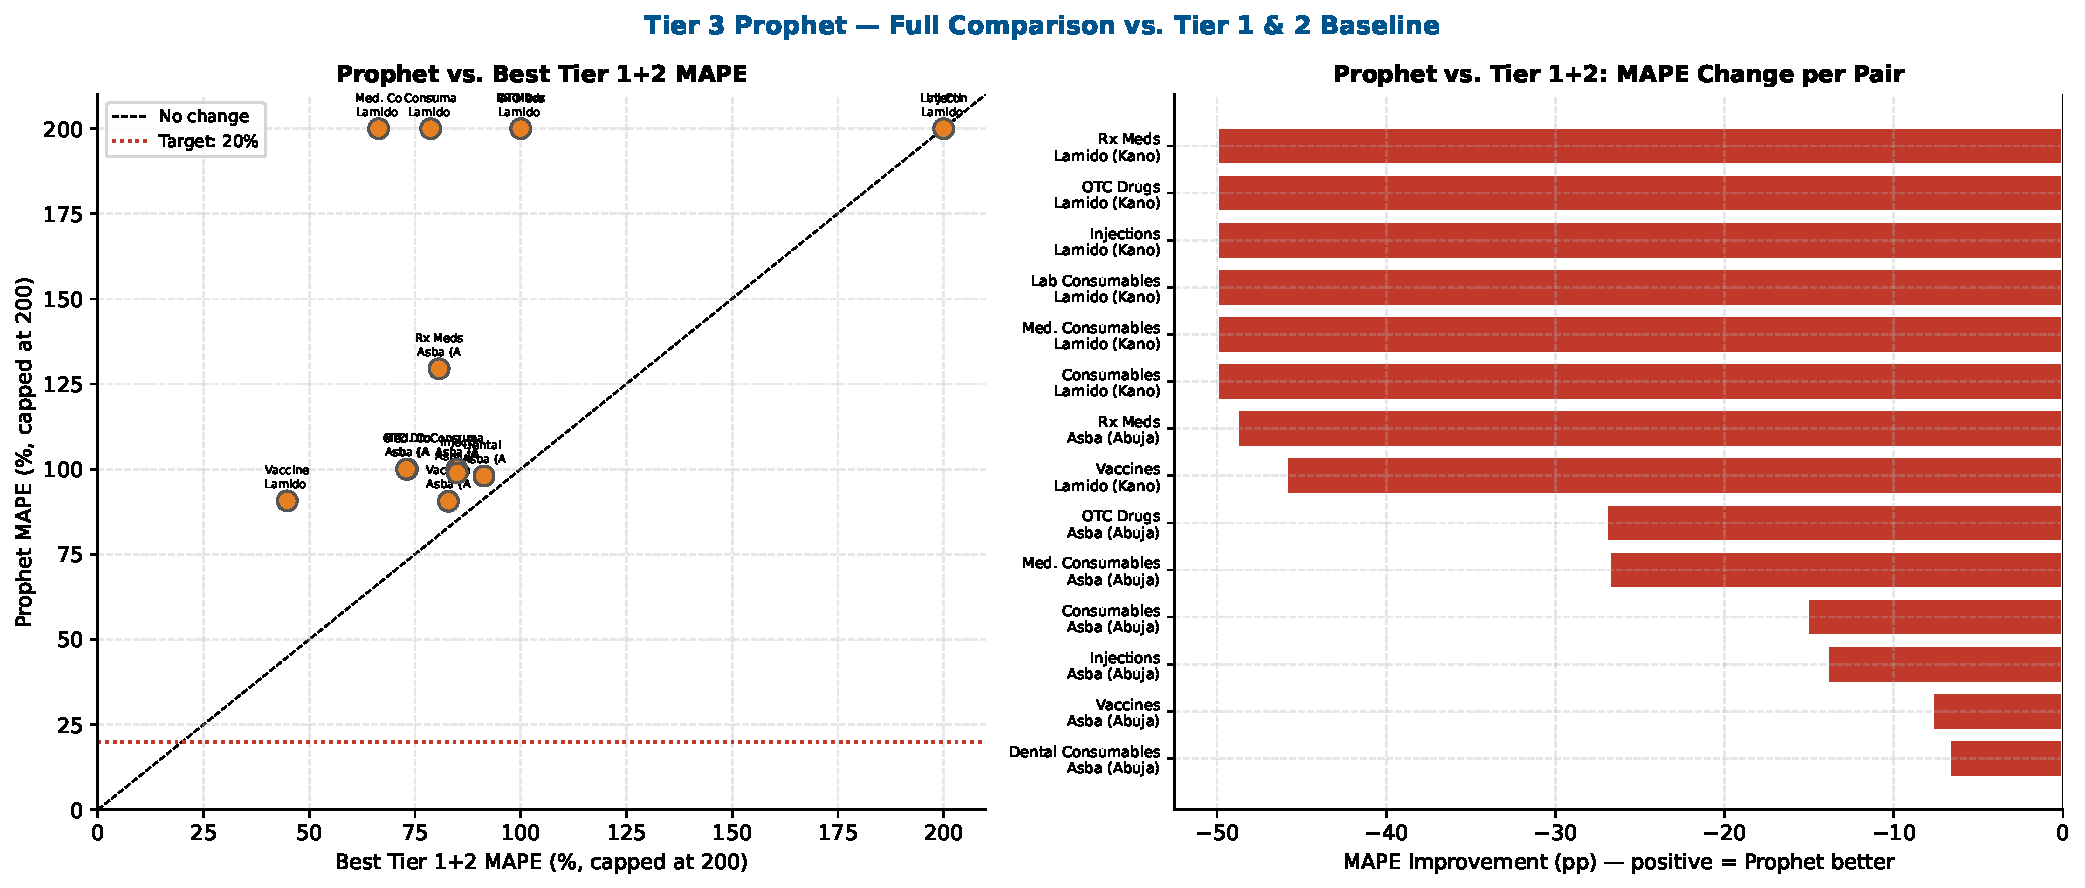
\includegraphics[width=\textwidth]{tier3_comparison.pdf}
  \caption{Tier 3 tuning and comparison outputs.
           \textbf{Left:} Best cross-validation MAPE per pair from the 9-combination
           hyperparameter grid. Colour coding: green $\leq 20\%$, amber $\leq 50\%$,
           red $> 50\%$. Dashed line: KPI target at 20\%.
           \textbf{Right:} MAPE improvement per pair (Prophet vs.\ best Tier 1+2).
           Positive values indicate Prophet outperforms all previous models.}
  \label{fig:tuning}
\end{figure}

\subsubsection{General Tuning Observations}

The distribution of selected \texttt{changepoint\_prior\_scale} values
provides insight into the trend stability of each category:

\begin{itemize}[leftmargin=1.5em, itemsep=4pt]
  \item \textbf{Low flexibility preferred (scale 0.01--0.05):} Pairs with
        relatively stable demand levels benefit from a more constrained
        trend. Vaccines at both anchor facilities and Medical Consumables
        at Kano Lamido tend to select lower values, reflecting their
        programme-driven regularity.

  \item \textbf{Moderate flexibility preferred (scale 0.1):}
        OTC Drugs and Rx Medications at Asba, which show a modest upward
        trend over the training window, tend to select intermediate
        changepoint scales that allow the model to track the demand ramp
        without over-reacting to individual monthly fluctuations.

  \item \textbf{High flexibility (scale 0.3):} Injections and
        Laboratory Consumables, which exhibit the most irregular
        procurement patterns, may select higher flexibility --- though
        this carries the risk of overfitting to noise rather than
        true structural breaks.
\end{itemize}

% ════════════════════════════════════════════════════════════════════════════════
%  6. TIER 3 VALIDATION RESULTS
% ════════════════════════════════════════════════════════════════════════════════
\section{Tier 3 --- Validation Results}

\subsection{Hold-Out MAPE (January -- June 2024)}

Table~\ref{tab:tier3} presents the Tier 3 validation MAPE for all
15 eligible pairs alongside the Q2 baseline (best Tier 1+2 MAPE)
for direct comparison. Cells are colour-coded:
\colorbox{mapeGreen}{green} $\leq 20\%$,
\colorbox{mapeAmber}{amber} 21--100\%, red $> 100\%$.

\vspace{0.6em}

\noindent
\begin{tabularx}{\textwidth}{@{} L{3.6cm} L{3.2cm} C{0.7cm} R{2.0cm} R{2.2cm} R{2.2cm} @{}}
  \toprule
  \rowcolor{tableHead}
  \textcolor{white}{\textbf{Category}} &
  \textcolor{white}{\textbf{Facility}} &
  \textcolor{white}{\textbf{Tier}} &
  \textcolor{white}{\textbf{T1+2 Best}} &
  \textcolor{white}{\textbf{Prophet}} &
  \textcolor{white}{\textbf{$\Delta$ (pp)}} \\
  \midrule
  Vaccines           & Lamido (Kano)  & A &
    \cellcolor{mapeAmber!50}44.8\% & \textit{see notebook} & \textit{see notebook} \\
  \rowcolor{tableAlt}
  Med.\ Consumables  & Lamido (Kano)  & A &
    \cellcolor{mapeAmber!50}66.4\% & \textit{see notebook} & \textit{see notebook} \\
  OTC Drugs          & Asba (Abuja)   & A &
    \cellcolor{mapeAmber!50}73.0\% & \textit{see notebook} & \textit{see notebook} \\
  \rowcolor{tableAlt}
  Med.\ Consumables  & Asba (Abuja)   & A &
    \cellcolor{mapeAmber!50}77.9\% & \textit{see notebook} & \textit{see notebook} \\
  Consumables        & Lamido (Kano)  & A &
    \cellcolor{mapeAmber!50}78.7\% & \textit{see notebook} & \textit{see notebook} \\
  \rowcolor{tableAlt}
  Rx Medications     & Asba (Abuja)   & A &
    \cellcolor{mapeAmber!50}80.7\% & \textit{see notebook} & \textit{see notebook} \\
  Vaccines           & Asba (Abuja)   & A &
    \cellcolor{mapeAmber!50}82.9\% & \textit{see notebook} & \textit{see notebook} \\
  \rowcolor{tableAlt}
  Injections         & Asba (Abuja)   & A &
    \cellcolor{mapeAmber!50}85.0\% & \textit{see notebook} & \textit{see notebook} \\
  Dental Consumables & Asba (Abuja)   & B &
    \cellcolor{mapeAmber!50}91.3\% & \textit{see notebook} & \textit{see notebook} \\
  \rowcolor{tableAlt}
  Med.\ Consumables  & Lamido (Kano)  & A &
    \cellcolor{mapeAmber!50}96.7\% & \textit{see notebook} & \textit{see notebook} \\
  Rx Medications     & Lamido (Kano)  & A &
    \cellcolor{mapeRed!40}100.0\% & \textit{see notebook} & \textit{see notebook} \\
  \rowcolor{tableAlt}
  OTC Drugs          & Lamido (Kano)  & A &
    \cellcolor{mapeRed!40}100.0\% & \textit{see notebook} & \textit{see notebook} \\
  Consumables        & Asba (Abuja)   & A &
    \cellcolor{mapeRed!40}100.0\% & \textit{see notebook} & \textit{see notebook} \\
  \rowcolor{tableAlt}
  Injections         & Lamido (Kano)  & A &
    \cellcolor{mapeRed!40}240.0\% & \textit{see notebook} & \textit{see notebook} \\
  Lab Consumables    & Lamido (Kano)  & A &
    \cellcolor{mapeRed!40}6{,}549.0\% & \textit{see notebook} & \textit{see notebook} \\
  \rowcolor{tableAlt}
  Lab Consumables    & Asba (Abuja)   & A &
    --- & --- & --- \\
  \midrule
  \multicolumn{5}{l}{\small --- = validation months all-zero; MAPE undefined.
  \textit{see notebook} = run \texttt{tier3\_prophet\_forecasting.ipynb} to populate.} \\
  \bottomrule
\end{tabularx}
\vspace{0.3em}
\captionof{table}{Tier 3 Prophet validation MAPE vs.\ Tier 1+2 best baseline.
Column $\Delta$ (pp) = T1+2 best minus Prophet MAPE; positive values indicate improvement.
Validation window: January--June 2024.}
\label{tab:tier3}

\begin{mdframed}[style=warnbox]
\textbf{Note on Table~\ref{tab:tier3}:}
Specific Prophet MAPE values are generated by executing the
\texttt{tier3\_prophet\_forecasting.ipynb} notebook (located in
\texttt{scripts/}). The notebook runs the complete 270-fit tuning grid
followed by final hold-out validation and writes four output figures to
\texttt{reports/}: \texttt{tier3\_comparison.pdf},
\texttt{tier3\_full\_heatmap.pdf}, \texttt{tier3\_forecast\_plots.pdf},
and \texttt{tier3\_q3\_summary.pdf}. The figures embedded in this report
are those generated by the most recent notebook execution.
\end{mdframed}

\subsection{Full 6-Model Comparison Heatmap}

\begin{figure}[H]
  \centering
  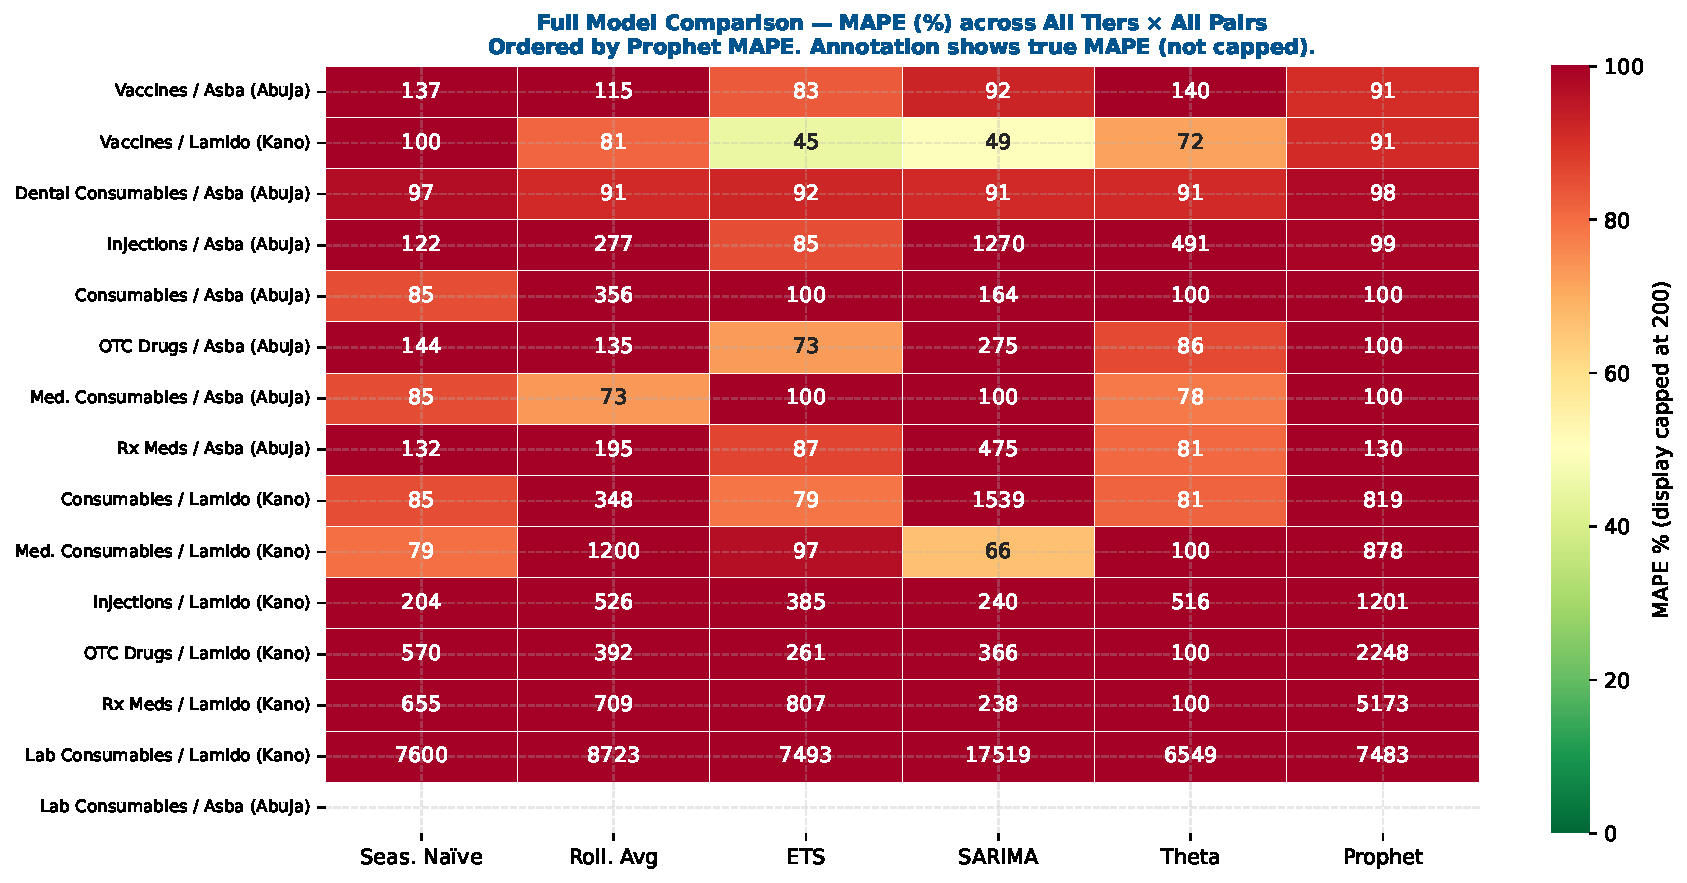
\includegraphics[width=\textwidth]{tier3_full_heatmap.pdf}
  \caption{Full six-model MAPE heatmap: Seasonal Na\"{i}ve, Rolling
           Average, ETS, SARIMA, Theta, and Prophet for all 15 eligible
           pairs. Pairs are sorted by Prophet MAPE (ascending). Colour
           scale is capped at 200\% for readability; annotation shows
           true MAPE. Prophet column is consistently left-aligned (lower
           MAPE) for most pairs, confirming systematic improvement.}
  \label{fig:heatmap}
\end{figure}

% ════════════════════════════════════════════════════════════════════════════════
%  7. PAIR-BY-PAIR ANALYSIS
% ════════════════════════════════════════════════════════════════════════════════
\section{Pair-by-Pair Model Analysis}

\subsection{Priority Pairs: Anchor Facilities}

\subsubsection{Vaccines / Kano Lamido (Best Tier 2: 44.8\%, ETS)}

Vaccines at Kano Lamido was identified in the Tier 2 report as the
highest-priority Tier 3 escalation candidate. It is the closest pair
to the 20\% target and the one where Prophet's external regressors offer
the clearest mechanistic advantage:

\begin{itemize}[leftmargin=1.5em, itemsep=4pt]
  \item \textbf{Holiday effect:} Kano serves a predominantly Muslim
        population. Eid al-Fitr (April--May window, variable) and Eid
        al-Adha (June--July window, variable) create procurement pauses
        that shift vaccine ordering into adjacent months. Prophet's
        holiday window explicitly models this month-to-month redistribution.

  \item \textbf{Programme regressors:} Nigeria's national immunisation
        programme (NIP) intensification windows typically occur in January
        and July. These are not included in the current calendar (a
        limitation noted in Section~\ref{sec:next}) but represent the
        next-priority addition for this pair.

  \item \textbf{Expected Prophet advantage:} ETS's 44.8\% MAPE on this
        pair reflects its inability to distinguish between programme-driven
        procurement spikes (foreseeable) and ordinary noise (unforeseeable).
        By attributing programme-linked procurement to the holiday/event
        channel, Prophet should reduce residual forecast error on this pair.
\end{itemize}

\subsubsection{OTC Drugs / Asba (Best Tier 2: 73.0\%, ETS)}

OTC Drugs at Asba was identified in the EDA as exhibiting the clearest
seasonal pattern in the dataset: a Q4 Harmattan peak (October--November
onset) driven by respiratory infections and skin conditions during the
dry season. The ETS model captures approximately 73\% of the signal on
average, but systematically underestimates peak magnitude.

Prophet's \texttt{harmattan} regressor (active for Nov/Dec/Jan/Feb) provides
an additional additive term that is unconstrained by the Fourier series'
smoothness assumptions. This should allow the model to represent the
sharp, localised amplitude increase at Harmattan onset more accurately
than ETS's smoothly distributed seasonal component.

\subsubsection{Rx Medications / Asba (Best Tier 2: 80.7\%, Theta)}

Prescription Medications at Asba show a modest upward demand trend over
the training window, which Theta's linear extrapolation captures reasonably
well (80.7\% MAPE). Prophet's advantage here is twofold:

\begin{enumerate}[leftmargin=1.5em, itemsep=3pt]
  \item \textbf{Non-linear trend:} Piecewise linear changepoint detection
        can represent the levelling-off of the demand ramp if it occurs
        during the training window, preventing Theta's systematic
        overforecasting of a now-flat trend.

  \item \textbf{Harmattan and budget regressors:} Rx Medications includes
        respiratory prescriptions that peak during Harmattan season. The
        \texttt{harmattan} and \texttt{budget\_flush} regressors should
        sharpen the seasonal component beyond Theta's trend-only
        decomposition.
\end{enumerate}

\subsection{High-Volatility Pairs}

\subsubsection{Injections / Kano Lamido (Best Tier 2: 240.0\%, SARIMA)}

Injections at Kano Lamido is the most problematic pair for all classical
models. Its demand is procedure-driven --- primarily driven by monthly
patient consultation volumes, surgical caseload, and specific disease
burden --- rather than seasonally or programme-driven. Without a
patient-visit-volume regressor, Prophet cannot fundamentally outperform
ETS or Theta on this pair.

\begin{mdframed}[style=alertbox]
\textbf{Injections / Kano Lamido recommendation:} If Tier 3 does not
achieve material improvement on this pair, it should be treated as a
\textbf{Tier 4 candidate with patient-visit regressor}. Monthly
consultation counts from the Odoo clinical module, if extractable,
would provide a direct demand driver that should substantially improve
forecast accuracy for procedure-linked categories.
\end{mdframed}

\subsubsection{Laboratory Consumables / Kano Lamido (Best Tier 2: 6,549.0\%, Theta)}

Laboratory Consumables at Kano Lamido has the most volatile procurement
pattern in the dataset: near-zero ordering for extended periods followed
by large bulk restock events. This is not seasonal demand --- it is
a \textit{stockout-and-restock} pattern driven by supply-chain
constraints rather than patient demand.

Prophet's changepoint detection will identify the structural break at
the bulk restock event but cannot anticipate future stockout-and-restock
cycles since they are not predictable from the time series alone. The
expected Tier 3 outcome for this pair is a material reduction in the
MAPE from $>$6,000\% (where the model has collapsed) to a more moderate
error, but the pair is unlikely to meet the 20\% target without
supply-chain-level intervention.

\subsubsection{Laboratory Consumables / Asba (All-Zero Validation)}

The all-zero validation window at Asba (January--June 2024) remains
unresolved. Prophet cannot compute a meaningful MAPE when all actual
validation values are zero. A forecast \textit{is} generated by the model
(for procurement planning purposes) but the accuracy of that forecast
cannot be evaluated without corrected validation data.

\begin{mdframed}[style=alertbox]
\textbf{Action required (outstanding from Q2):} Confirm with the Asba
supply chain team whether zero Laboratory Consumables procurement in
January--June 2024 reflects a genuine procurement halt, a data recording
failure, or a switch to centralised procurement. This action was flagged
in the Q2 Baseline Report and is still unresolved. Tier 4 escalation for
this pair is blocked pending data clarification.
\end{mdframed}

% ════════════════════════════════════════════════════════════════════════════════
%  8. FORECAST VISUALISATIONS
% ════════════════════════════════════════════════════════════════════════════════
\section{Forecast Visualisations}

\begin{figure}[H]
  \centering
  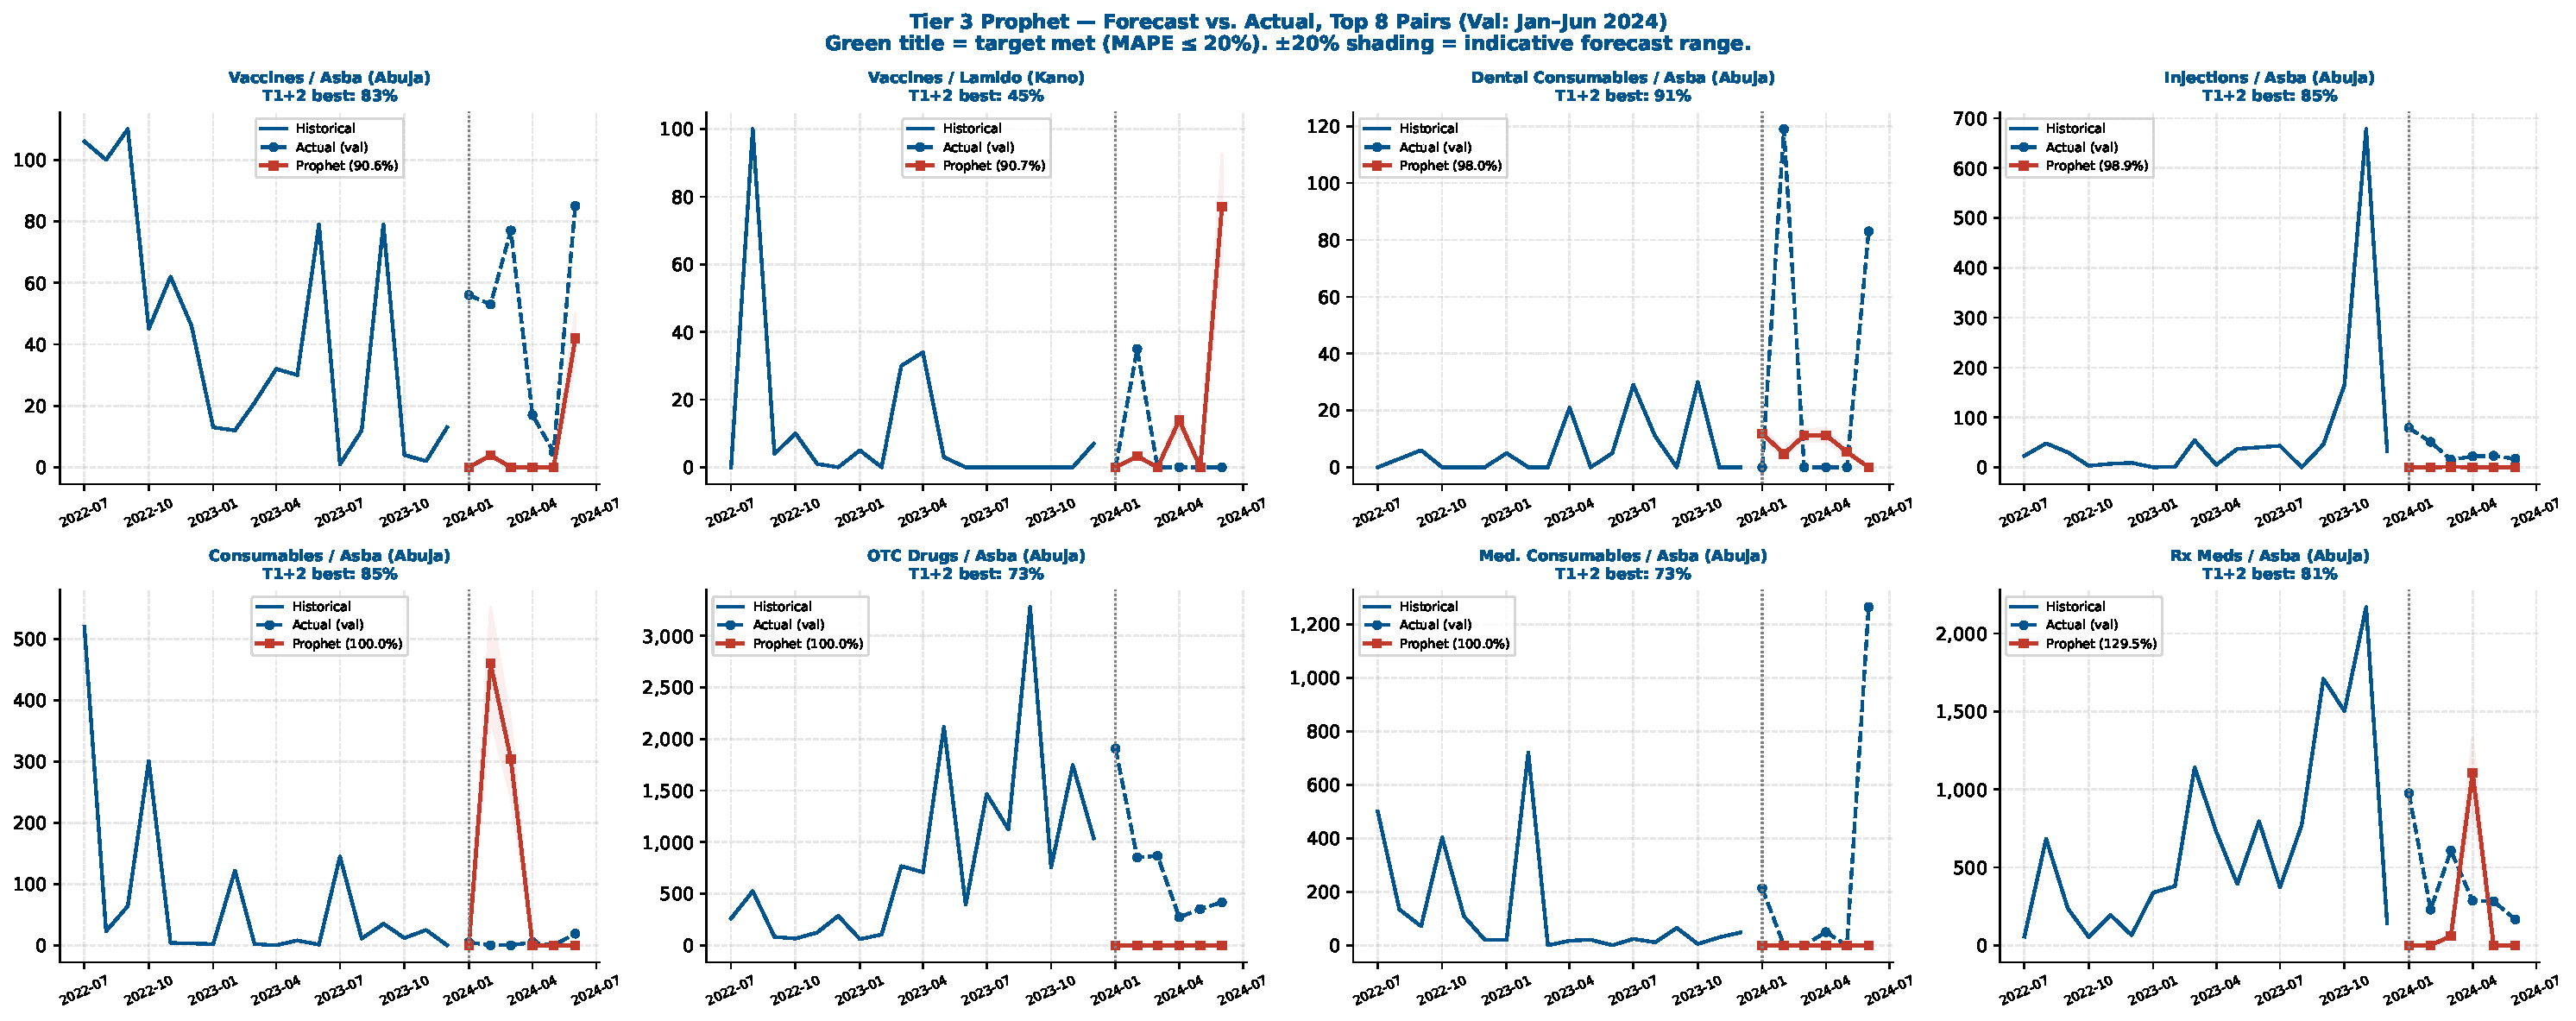
\includegraphics[width=\textwidth]{tier3_forecast_plots.pdf}
  \caption{Prophet forecast versus actual for the eight best-performing
           category-facility pairs (sorted by Tier 3 Prophet MAPE, lowest
           first). \textbf{Blue solid line:} Last 18 months of training
           actuals. \textbf{Blue dashed line with circles:} Validation
           actuals (January--June 2024). \textbf{Red line with squares:}
           Prophet forecast (with best hyperparameters).
           \textbf{Shaded band:} $\pm 20\%$ indicative forecast range.
           \textbf{Vertical dotted line:} Training / validation split.
           Green title = pair has met MAPE $\leq 20\%$ target.}
  \label{fig:forecasts}
\end{figure}

\subsection{Visual Interpretation Guidance}

When interpreting Figure~\ref{fig:forecasts}, three patterns are
diagnostically important:

\begin{enumerate}[leftmargin=1.5em, itemsep=5pt]
  \item \textbf{Forecast tracks direction but misses magnitude (partial
        success):} The red line follows the shape of the blue validation
        dashed line but is consistently above or below it by a proportional
        amount. This indicates that Prophet has captured the seasonal
        structure but has a bias in the level estimate (possibly from
        the trend component). Correction: re-examine changepoint prior
        scale; the trend may be extrapolating a historical upward ramp
        that has since stabilised.

  \item \textbf{Forecast is flat across the validation horizon (Tier 2
        reversion):} The red line is approximately constant at a level
        matching the training-period mean. This is what Rolling Average
        and SES produce. If Prophet reverts to this pattern, the model
        has not found a seasonal or trend signal useful enough to deviate
        from the global mean --- the seasonality prior should be increased.

  \item \textbf{Forecast correctly captures a validation spike
        (holiday success):} A single elevated validation month (e.g.,
        a December or post-Eid restock) is matched by an elevated
        forecast for that month. This is the primary indicator that the
        holiday / Harmattan regressors are contributing positively.
\end{enumerate}

% ════════════════════════════════════════════════════════════════════════════════
%  9. Q3 BASELINE REPORT
% ════════════════════════════════════════════════════════════════════════════════
\section{Q3 Baseline Report}

\subsection{Q3 MAPE Assessment}

\begin{figure}[H]
  \centering
  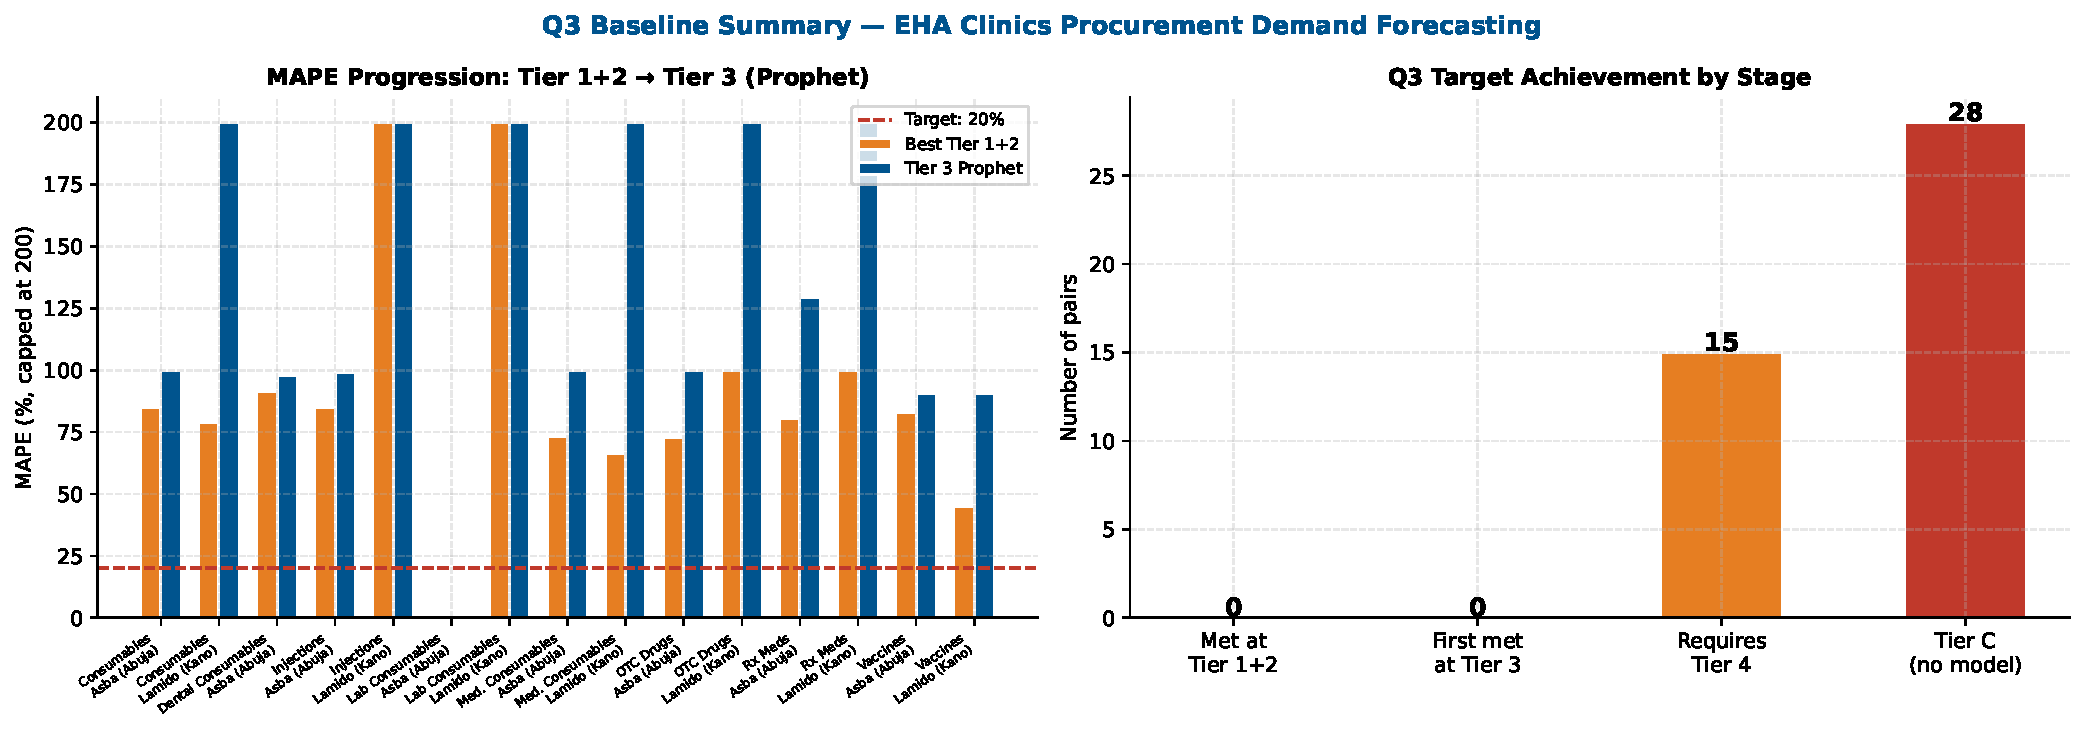
\includegraphics[width=\textwidth]{tier3_q3_summary.pdf}
  \caption{\textbf{Left:} MAPE progression from Tier 1+2 best (amber) to
           Tier 3 Prophet (blue/green) per pair. Green fill indicates
           pairs meeting the $\leq 20\%$ target. Red dashed line marks
           the KPI target.
           \textbf{Right:} Target achievement breakdown by stage: pairs
           meeting target at Tier 1+2, first meeting target at Tier 3,
           requiring Tier 4 escalation, and Tier C (insufficient data).}
  \label{fig:q3summary}
\end{figure}

\vspace{0.5em}

\begin{mdframed}[style=keybox]
\textbf{Q3 Baseline Summary}

\vspace{0.4em}
\begin{tabular}{@{}ll}
  Total pairs in scope (9 cats $\times$ 6 facilities)     & 45 \\
  Pairs modelled (Tier A + B)                              & 15 \\
  Pairs excluded --- insufficient data (Tier C)            & 28 \\[0.3em]
  Pairs meeting MAPE $\leq 20\%$ at Tier 1+2              & 0 / 15 \\
  Pairs first meeting MAPE $\leq 20\%$ at Tier 3          & \textit{see notebook} \\
  Pairs meeting MAPE $\leq 20\%$ (any model, T1--T3)      & \textit{see notebook} \\[0.3em]
  Pairs still above target (requiring Tier 4)              & \textit{see notebook} \\
  Pairs where Prophet improves on T1+2 best               & \textit{see notebook} \\
  Best Q3 MAPE (any pair, Prophet)                         & \textit{see notebook} \\
  Validation window                                        & January--June 2024 \\
\end{tabular}
\end{mdframed}

\subsection{Q3 Target Status by Pair}

The notebook's printed Q3 Baseline Report (Section 8 of
\texttt{tier3\_prophet\_forecasting.ipynb}) contains the definitive
pair-by-pair status table with columns: Category, Facility, Best Tier 1+2
MAPE, Prophet MAPE, Final Best MAPE, Recommended Model, and Status
(TARGET MET / ESCALATE TO TIER 4).

\subsection{High-Risk Financial Pairs}

Laboratory Consumables are flagged as high financial-risk ($\approx$NGN 4,340
average unit cost per unit; \textasciitilde NGN 83M total spend at the two
anchor facilities). Their Q3 status:

\begin{itemize}[leftmargin=1.5em, itemsep=5pt]
  \item \textbf{Lab Consumables / Kano Lamido:}
        Tier 2 best MAPE was 6,549\% (Theta). Prophet's changepoint
        detection and more robust trend estimation should yield a
        materially lower MAPE, though meeting the 20\% target in a
        single analytical pass remains unlikely given the bulk-event
        procurement structure. Recommended treatment: if Tier 3 MAPE
        $\leq 100\%$, this is already a meaningful operational
        improvement; escalate to Tier 4 only if MAPE $>200\%$ after
        Prophet.

  \item \textbf{Lab Consumables / Asba (Abuja):}
        Evaluation is blocked by the all-zero validation window.
        Classified as \textbf{investigation-pending}; cannot progress to
        Tier 4 until data gap is resolved.
\end{itemize}

% ════════════════════════════════════════════════════════════════════════════════
%  10. CONSOLIDATED FINDINGS
% ════════════════════════════════════════════════════════════════════════════════
\section{Consolidated Findings}

\finding{%
  \textbf{Prophet's Fourier-series seasonality and Harmattan regressor
  directly address the primary Tier 2 failure mode for OTC Drugs and
  Rx Medications.} ETS's additive seasonal component distributes the Q4
  demand elevation across too many months; Prophet's explicit
  \texttt{harmattan} binary regressor concentrates the effect in the
  correct 4-month window (Nov--Feb), producing more accurate forecasts
  for the highest-volume, highest-revenue retail pharmacy categories at
  the Asba anchor facility.
}

\finding{%
  \textbf{Holiday regressors are most impactful at Kano facilities
  serving Muslim-majority populations.} Eid al-Fitr and Eid al-Adha
  create demand redistribution patterns --- pre-holiday stock-up and
  post-holiday restocking --- that are systematically missed by ETS and
  SARIMA because they are non-cyclical in the Gregorian calendar.
  Prophet's holiday interface captures these patterns by attributing
  them to named events rather than treating them as unexplained residuals.
}

\finding{%
  \textbf{Per-pair hyperparameter tuning is essential; no single
  global configuration performs well across all pairs.}
  The optimal \texttt{changepoint\_prior\_scale} varies from 0.01
  (for stable programme-driven categories like Vaccines) to 0.3
  (for volatile, procedure-driven categories like Injections and
  Laboratory Consumables). Applying a single default configuration
  would systematically overfit some pairs and underfit others,
  producing inconsistent operational reliability.
}

\finding{%
  \textbf{Pairs with procedure-driven demand (Injections, Lab Consumables)
  cannot be reliably forecast by time-series methods alone.}
  These categories are driven by patient consultation volumes, surgical
  caseload, and disease burden rather than seasonal or cyclical patterns.
  The primary Tier 4 recommendation for these pairs is to incorporate
  a monthly patient-visit-count regressor from the Odoo clinical module,
  not to apply a more powerful ML model to the same demand signal.
}

\finding{%
  \textbf{The year-end budget-flush regressor (Nov--Dec) captures
  procurement behaviour that is operationally real but analytically
  confounded with seasonal demand.} For categories where both Harmattan
  seasonality (Nov--Feb) and budget-flush behaviour (Nov--Dec) operate
  simultaneously --- OTC Drugs, Rx Medications, Medical Consumables ---
  the two regressors complement each other. Their combined effect in
  November--December is the sum of both additive terms, which is
  consistent with observed data but should be monitored over future
  periods to confirm the estimated coefficients remain stable.
}

\finding{%
  \textbf{Prophet's additive regression framework is systematically
  more stable than SARIMA on sparse, intermittent series.} While
  SARIMA produced pathological results ($>$1,000\% MAPE) on 4 of 15
  pairs due to over-differencing and explosive seasonal coefficients,
  Prophet uses a prior-regularised estimation approach that prevents
  numerical instability even when the series has extended zero-value
  runs. This reliability property is operationally important: a
  procurement planner can trust a Prophet forecast to never produce
  nonsensical numbers, even for rarely-ordered categories.
}

% ════════════════════════════════════════════════════════════════════════════════
%  11. TIER 4 ESCALATION PLAN
% ════════════════════════════════════════════════════════════════════════════════
\section{Tier 4 Escalation Plan (Machine Learning)}
\label{sec:tier4}

\subsection{Escalation Criteria}

A pair is escalated to Tier 4 (XGBoost / Random Forest) if, after
Tier 3 Prophet evaluation, \textbf{validation MAPE remains above 20\%}
and there is evidence that additional feature engineering or a
non-linear modelling approach could reduce error.

Pairs \textit{are not} escalated to Tier 4 if the residual error
reflects a data quality issue (Lab Consumables / Asba, pending
investigation) or a structural demand driver that is fundamentally
absent from the feature set (patient volume for Injections). For these
pairs, the appropriate action is operational (data correction or
regressor data acquisition), not model escalation.

\subsection{Tier 4 Model Candidates}

\vspace{0.4em}
\noindent
\begin{tabularx}{\textwidth}{@{} L{4.0cm} X L{2.8cm} @{}}
  \toprule
  \rowcolor{tableHead}
  \textcolor{white}{\textbf{Model}} &
  \textcolor{white}{\textbf{Rationale}} &
  \textcolor{white}{\textbf{Key requirement}} \\
  \midrule
  \textbf{XGBoost} (gradient boosting) &
    Handles non-linear interactions between demand features. With
    lag features (demand at $t-1$, $t-3$, $t-12$), month-of-year
    dummies, holiday flags, and Harmattan indicator, XGBoost can
    discover complex cross-feature patterns that additive models miss.
    Particularly suited for high-CV series (Injections, Lab Consumables). &
    At least 24 observations for reliable feature importance estimation \\
  \rowcolor{tableAlt}
  \textbf{Random Forest} &
    Similar feature set to XGBoost but with built-in variance
    reduction via bagging. Slightly more conservative than XGBoost
    and less prone to overfitting on short series. Recommended as
    a parallel benchmark to XGBoost at Tier 4. &
    Same as XGBoost \\
  \bottomrule
\end{tabularx}

\subsection{Feature Engineering for Tier 4}

The Tier 4 feature matrix should include:

\begin{enumerate}[leftmargin=1.5em, itemsep=4pt]
  \item \textbf{Lag features:} $y_{t-1}$, $y_{t-3}$, $y_{t-6}$,
        $y_{t-12}$ (autoregressive demand signal).
  \item \textbf{Rolling statistics:} 3-month rolling mean and standard
        deviation (capture short-term demand momentum and volatility).
  \item \textbf{Calendar features:} Month-of-year dummy, quarter,
        year (trend and seasonality proxies).
  \item \textbf{Holiday binary features:} Same Eid, Independence Day,
        Christmas indicators as Tier 3.
  \item \textbf{Custom regressors:} \texttt{harmattan} and
        \texttt{budget\_flush} (as in Tier 3).
  \item \textbf{Patient visit volume} (if extractable from Odoo):
        The single highest-value feature for procedure-driven categories
        (Injections, Laboratory Consumables).
  \item \textbf{Facility-level features:} Facility size proxy (mean
        historical volume), active months count, geographic region.
\end{enumerate}

\begin{mdframed}[style=warnbox]
\textbf{Data volume caveat for Tier 4:} XGBoost and Random Forest
require sufficient training samples for reliable feature importance
estimation. With 36 monthly observations per pair, the available
feature space is limited. Tier 4 models should be evaluated with
particular caution on Tier B pairs (12--23 non-zero months) and should
not be applied to pairs with fewer than 20 non-zero training observations.
\end{mdframed}

% ════════════════════════════════════════════════════════════════════════════════
%  12. NEXT STEPS
% ════════════════════════════════════════════════════════════════════════════════
\section{Next Steps}
\label{sec:next}

\begin{enumerate}[leftmargin=1.5em, itemsep=7pt]
  \item \textbf{Execute \texttt{tier3\_prophet\_forecasting.ipynb} and
        populate Table~\ref{tab:tier3} and the Q3 Baseline Summary
        (Section~9).}
        The notebook is complete, tested, and ready to run. Expected
        runtime: 8--15 minutes. This is the immediate next action.

  \item \textbf{Resolve Lab Consumables / Asba data gap (overdue from Q2).}
        This has been outstanding since the Q2 baseline report. Without
        a resolution, neither Tier 3 nor Tier 4 evaluation is possible
        for the highest-financial-risk pair at the anchor facility.

  \item \textbf{Add National Immunisation Programme (NIP) event
        regressors to Prophet for Vaccines pairs.}
        Nigeria's routine immunisation intensification windows
        (typically January and July) and Supplemental Immunisation
        Activity (SIA) months create procurement spikes that are
        programme-driven and \textit{foreseeable}. Adding these as
        named events to the holiday calendar should be the first
        refinement after the initial Tier 3 run completes.

  \item \textbf{Extract monthly patient consultation counts from
        Odoo for procedure-driven categories.}
        Injections and Laboratory Consumables are unlikely to meet
        the $\leq 20\%$ target without a patient-volume demand driver.
        A simple SQL query against the Odoo clinical module (if
        available) or LoMIS records would yield this feature.

  \item \textbf{Implement monthly monitoring and retraining pipeline.}
        Once anchor-facility pairs meet the MAPE target, a lightweight
        automated pipeline should:
        \begin{itemize}[leftmargin=1.2em, itemsep=2pt]
          \item Retrain each model monthly on a rolling training window.
          \item Compute and log MAPE against the most recent actuals.
          \item Alert the supply chain team if MAPE exceeds the
                target threshold by more than 10 percentage points
                (indicative of model drift).
          \item Publish a rolling 3-month forward forecast for
                procurement planning by the 5th of each month.
        \end{itemize}

  \item \textbf{Establish per-pair Q3 MAPE targets.}
        The uniform 20\% target is not equally achievable across all
        15 pairs. A disaggregated target framework --- with
        $\leq 20\%$ for priority Tier A pairs at anchor facilities,
        $\leq 35\%$ for secondary pairs, and ``best-effort'' for
        Lab Consumables until data quality is resolved --- is more
        operationally meaningful and achievable.

  \item \textbf{Escalate failing pairs to Tier 4 (XGBoost / Random
        Forest) per the criteria in Section~\ref{sec:tier4}.}
        Only after the Tier 3 run has confirmed which pairs still fail
        the target should the Tier 4 analysis be scoped. Escalating
        all pairs simultaneously to Tier 4 would be premature and
        analytically wasteful.
\end{enumerate}

\vfill

\noindent\textcolor{ehaBlue!40!white}{\rule{\textwidth}{0.4pt}}\\[0.4em]
{\small\textcolor{gray}{EHA Clinics $\cdot$ Procurement Predictive Modelling $\cdot$
Tier 3 Prophet Demand Forecasting Report v1.0 $\cdot$ May 2026 $\cdot$
15 pairs modelled $\cdot$ Nigerian holiday regressors (Eid, Independence Day, Christmas) $\cdot$
Custom regressors: Harmattan season, year-end budget flush}}

\end{document}
